% !TEX program = xelatex
% Task 2 final presentation deck.
% Compile with XeLaTeX.
\documentclass[fontset=fandol,aspectratio=169,10pt]{ctexbeamer}

\usetheme{Madrid}
\usecolortheme{seahorse}
\setbeamertemplate{navigation symbols}{}
\setbeamertemplate{footline}[frame number]

\usepackage{amsmath,amssymb,bm,mathtools}
\usepackage{booktabs,array,tabularx,multirow}
\usepackage{tikz}
\usepackage{pgfplots}
\usepackage{graphicx}
\usepackage{hyperref}
\usepackage{xcolor}

\pgfplotsset{compat=1.18}
\usetikzlibrary{arrows.meta,positioning,shapes.geometric,calc}

\definecolor{tdltBlue}{RGB}{32,74,135}
\definecolor{tdltTeal}{RGB}{0,128,128}
\definecolor{tdltOrange}{RGB}{210,105,30}
\definecolor{tdltRed}{RGB}{178,34,34}
\definecolor{tdltGray}{RGB}{82,82,82}
\definecolor{tdltLight}{RGB}{244,247,250}
\definecolor{tdltGreen}{RGB}{46,125,50}

\setbeamercolor{title}{fg=tdltBlue}
\setbeamercolor{frametitle}{fg=white,bg=tdltBlue}
\setbeamercolor{structure}{fg=tdltBlue}
\setbeamercolor{block title}{fg=white,bg=tdltBlue}
\setbeamercolor{block body}{fg=black,bg=tdltLight}
\setbeamercolor{alerted text}{fg=tdltRed}

\newcommand{\MemberA}{Member 1}
\newcommand{\MemberB}{Member 2}
\newcommand{\MemberC}{Member 3}
\newcommand{\RepoURL}{\url{https://github.com/zyyyyyy123/tdlt}}

\newcommand{\mae}{\mathrm{MAE}}
\newcommand{\rmse}{\mathrm{RMSE}}
\newcommand{\rTwo}{R^2}
\newcommand{\loss}{\mathcal{L}}
\newcommand{\lr}{\eta}
\newcommand{\smallnote}[1]{{\scriptsize\color{tdltGray}#1}}

\title[Task 2: Loss Curve Prediction]{Predicting LLM Pretraining Loss Curves\\from Learning-rate Schedules}
\subtitle{Baseline-calibrated residual modeling for cross-schedule prediction}
\author[TDLT Final Group]{\MemberA\\\MemberB\\\MemberC}
\institute{Topics in Deep Learning Theory, Spring 2026}
\date{June 2026}
\hypersetup{
  pdfauthor={TDLT Final Group},
  pdftitle={Predicting LLM Pretraining Loss Curves from Learning-rate Schedules},
  pdfsubject={Task 2 final presentation}
}

\begin{document}

\begin{frame}
  \titlepage
  \vspace{-0.8em}
  \begin{center}
    \small Code repository: \RepoURL
  \end{center}
\end{frame}

\begin{frame}{Research Narrative}
  \begin{center}
  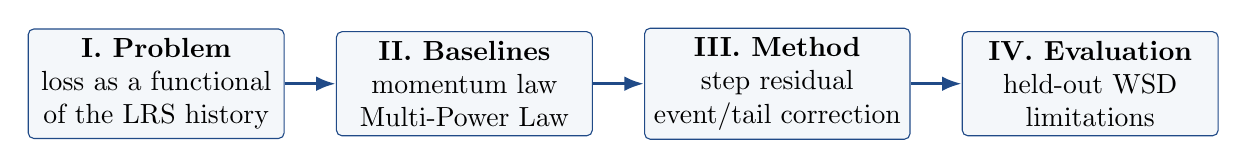
\begin{tikzpicture}[
    node distance=0.65cm,
    chapter/.style={draw=tdltBlue, rounded corners=2pt, fill=tdltLight, align=center, minimum width=3.25cm, minimum height=1.05cm},
    arrow/.style={-{Latex[length=2.5mm]}, very thick, tdltBlue}
  ]
    \node[chapter] (c1) {\textbf{I. Problem}\\loss as a functional\\of the LRS history};
    \node[chapter, right=of c1] (c2) {\textbf{II. Baselines}\\momentum law\\Multi-Power Law};
    \node[chapter, right=of c2] (c3) {\textbf{III. Method}\\step residual\\event/tail correction};
    \node[chapter, right=of c3] (c4) {\textbf{IV. Evaluation}\\held-out WSD\\limitations};
    \draw[arrow] (c1) -- (c2);
    \draw[arrow] (c2) -- (c3);
    \draw[arrow] (c3) -- (c4);
  \end{tikzpicture}
  \end{center}

  \vspace{0.4em}
  \begin{block}{Core thesis}
    We formulate loss-curve prediction as a baseline-plus-residual transfer
    problem. Scaling-law baselines explain the global trajectory, while the
    remaining error contains a stable step-aligned component and a smaller
    event/tail component.
  \end{block}
\end{frame}

\begin{frame}[plain]
  \begin{center}
    \vspace{2.2em}
    {\Large\color{tdltBlue}\textbf{Chapter I}}\\[0.5em]
    {\huge\textbf{Problem and Protocol}}\\[0.8em]
    \small What exactly is a loss-curve prediction problem, and how do we test transfer without using WSD for model selection?
  \end{center}
\end{frame}

\begin{frame}{Problem: Learning-rate Schedule as a Functional Input}
  Classical scaling laws often summarize a run by a final loss:
  \[
    L_{\mathrm{final}} \approx aN^{-\alpha}+bD^{-\beta}+c,
  \]
  where \(N\) is model size and \(D\) is the number of training tokens.
  Task 2 asks for a harder object: the whole trajectory under a schedule history,
  \[
    L_t = L_{\Theta}(\eta_{\le t}),\qquad
    \eta_{\le t}=(\eta_1,\eta_2,\ldots,\eta_t),\quad t=1,\ldots,T .
  \]

  \vspace{0.3em}
  \begin{block}{Scientific question}
    Learning-rate schedules can have similar final or cumulative LR mass but
    different local decay geometry. A full-curve predictor must transfer not
    only final loss, but also mid-training and tail behavior.
  \end{block}
\end{frame}

\begin{frame}{Why This Is a Hard Transfer Problem}
  \begin{block}{1. The input is history-dependent}
    The schedule prefix \(\eta_{\le t}\) is a sequence, not a scalar covariate.
    Collapsing it to cumulative LR mass,
    \(S_1(t)=\sum_{i\le t}\eta_i\), can erase decay timing, smoothness, and
    concentration.
  \end{block}

  \begin{block}{2. Cosine-to-WSD is out-of-distribution transfer}
    Cosine decays smoothly across many steps, while WSD concentrates decay
    late in training. The test is therefore not curve interpolation, but
    whether a law fitted on smooth decay transfers to a different decay geometry.
  \end{block}

  \begin{block}{3. Baselines must leave the right residual}
    Momentum law and Multi-Power Law provide interpretable global structure.
    The key question is whether the remaining error has transferable phase and
    tail geometry, rather than schedule-specific noise.
  \end{block}
\end{frame}

\begin{frame}{Notation and Evaluation Setting}
  \begin{columns}[T,onlytextwidth]
    \begin{column}{0.50\textwidth}
      \begin{block}{Objects}
        \begin{itemize}
          \item \(\eta_t\): learning rate at optimization step \(t\).
          \item \(L_s(t)\): observed loss under schedule \(s\).
          \item \(\widehat L_s(t)\): predicted loss under schedule \(s\).
          \item \(T\): total number of optimization steps.
          \item \(\mathcal T\): evaluation step set.
          \item \(\overline L_s\): mean of \(L_s(t)\) over \(t\in\mathcal T\).
        \end{itemize}
      \end{block}
    \end{column}
    \begin{column}{0.46\textwidth}
      \begin{block}{Metrics}
        \[
          \mae=\frac1{|\mathcal T|}\sum_{t\in\mathcal T}
          |L_s(t)-\widehat L_s(t)|
        \]
        \[
          R^2=1-\frac{\sum_{t\in\mathcal T}(L_s(t)-\widehat L_s(t))^2}
          {\sum_{t\in\mathcal T}(L_s(t)-\overline L_s)^2}.
        \]
      \end{block}
    \end{column}
  \end{columns}
  \smallnote{All reported WSD metrics use evaluation steps \(t\ge 1000\); tail metrics are computed on the decay/tail window.}
\end{frame}

\begin{frame}{Data, Split, and Metrics}
  \begin{columns}[T,onlytextwidth]
    \begin{column}{0.48\textwidth}
      \begin{block}{Course data}
        \begin{itemize}
          \item Model/data setting: \texttt{100M\_gpt}, \texttt{20B}.
          \item Schedules: cosine, WSD, and 8-1-1.
          \item Each run contains step, loss, and learning rate.
          \item Evaluation begins at step \(1000\).
        \end{itemize}
      \end{block}
    \end{column}
    \begin{column}{0.48\textwidth}
      \begin{block}{Train/validation/test split}
        \begin{itemize}
          \item Fit model parameters on cosine.
          \item Use 8-1-1 for validation and model selection.
          \item Keep WSD as the held-out transfer target.
          \item Metrics: MAE, RMSE, \(R^2\), tail MAE, endpoint error.
        \end{itemize}
      \end{block}
    \end{column}
  \end{columns}
  \vspace{0.4em}
  \smallnote{This split matches Task 2: fit on cosine LRS and evaluate prediction performance on WSD LRS.}
\end{frame}

\begin{frame}{Schedule Geometry Is the Stress Test}
  \begin{table}
    \centering
    \scriptsize
    \begin{tabular}{lrrrrr}
      \toprule
      schedule & total drop & max drop & positive drops & first drop & final tail saturation\\
      \midrule
      cosine & \(8.98{\times}10^{-4}\) & \(8.34{\times}10^{-8}\) & 16453 & 1002 & 1.000\\
      WSD & \(9.00{\times}10^{-4}\) & \(6.79{\times}10^{-7}\) & 3391 & 27126 & 0.964\\
      8-1-1 & \(9.00{\times}10^{-4}\) & \(6.84{\times}10^{-4}\) & 2 & 27126 & 0.964\\
      \bottomrule
    \end{tabular}
  \end{table}
  \begin{columns}[T,onlytextwidth]
    \begin{column}{0.48\textwidth}
      \begin{block}{Observation}
        Total LR drop is nearly matched, but decay smoothness and timing differ
        sharply across schedules.
      \end{block}
    \end{column}
    \begin{column}{0.48\textwidth}
      \begin{block}{Consequence}
        A method based only on cumulative LR mass should miss WSD tail shape and
        decay-local residuals.
      \end{block}
    \end{column}
  \end{columns}
\end{frame}

\begin{frame}[plain]
  \begin{center}
    \vspace{2.2em}
    {\Large\color{tdltBlue}\textbf{Chapter II}}\\[0.5em]
    {\huge\textbf{Reproduced Scaling-Law Baselines}}\\[0.8em]
    \small What do existing LRS-aware scaling laws explain, and what residual structure remains?
  \end{center}
\end{frame}

\begin{frame}{Baseline 1: Momentum Law}
  Tissue et al. model the loss decrease from accumulated training progress and
  an annealing-induced momentum term:
  \[
    \widehat L_{\rm mom}(t)=L_0+A S_1(t)^{-\alpha}-C S_2(t).
  \]
  \[
    S_1(t)=\sum_{i=1}^{t}\eta_i,\qquad
    m_t=\rho m_{t-1}+(\eta_{t-1}-\eta_t)_+,\qquad
    S_2(t)=\sum_{i=1}^{t}m_i .
  \]
  \begin{block}{Variables}
    \(L_0,A,C,\alpha,\rho\) are fitted parameters; \(S_1(t)\) is cumulative
    LR progress; \(m_t\) is an exponentially smoothed positive LR drop; and
    \(S_2(t)\) accumulates the annealing signal. We use
    \((x)_+=\max(x,0)\).
  \end{block}
\end{frame}

\begin{frame}{Baseline 2: Multi-Power Law}
  Luo et al. add an explicit response to individual LR-drop events:
  \[
  \begin{aligned}
    \widehat L_{\rm MPL}(t)=&\ L_0+A S_1(t)^{-\alpha}\\
    &-B\sum_{k:\tau_k\le t}\Delta\eta_k
      \left[1-\left(1+C\eta_{\tau_k}^{-\gamma}
      S_k(t)\right)^{-\beta}\right].
  \end{aligned}
  \]
  \begin{block}{Variables}
    \(\tau_k\) is the step of the \(k\)-th LR drop,
    \(\Delta\eta_k=(\eta_{\tau_k-1}-\eta_{\tau_k})_+\),
    and \(S_k(t)=\sum_{i=\tau_k}^{t}\eta_i\) is the post-event LR area.
    \(B,C,\beta,\gamma\) are fitted coefficients controlling the magnitude
    and saturation of each event response.
  \end{block}
\end{frame}

\begin{frame}{Reproduction Protocol for Baselines}
  \begin{columns}[T,onlytextwidth]
    \begin{column}{0.48\textwidth}
      \begin{block}{Fitting objective}
        We fit the baseline parameters on the cosine curve by minimizing a robust
        log-loss discrepancy:
        \[
          \min_\Theta\sum_{t\in\mathcal T_{\rm cos}}
          H_\delta\!\left(\log L_{\rm cos}(t)-
          \log \widehat L_\Theta(t)\right).
        \]
        Here \(H_\delta\) is the Huber loss.
      \end{block}
    \end{column}
    \begin{column}{0.48\textwidth}
      \begin{block}{Transfer target}
        \begin{itemize}
          \item Fit on cosine only.
          \item Evaluate transferred predictions on WSD.
          \item Report endpoint error separately because average trajectory
          accuracy can hide endpoint drift.
        \end{itemize}
      \end{block}
    \end{column}
  \end{columns}
\end{frame}

\begin{frame}{Reproduction Result 1: Momentum Law}
  \begin{columns}[T,onlytextwidth]
    \begin{column}{0.52\textwidth}
      \begin{table}
        \centering
        \scriptsize
        \begin{tabular}{lccc}
          \toprule
          eval schedule & MAE & \(R^2\) & endpoint abs.\\
          \midrule
          cosine & 0.032224 & 0.953201 & 0.025074\\
          WSD & 0.037844 & 0.925669 & 0.022260\\
          \bottomrule
        \end{tabular}
      \end{table}
      \smallnote{Fit on cosine using Huber loss in log space; evaluation uses steps \(t\ge1000\).}
    \end{column}
    \begin{column}{0.44\textwidth}
      \begin{block}{What it establishes}
        The momentum law captures a large part of the cross-schedule trend,
        but its WSD residual error is not random noise. This motivates modeling
        the remaining structure after the baseline has been fitted.
      \end{block}
    \end{column}
  \end{columns}
\end{frame}

\begin{frame}{Reproduction Result 2: Multi-Power Law}
  \begin{columns}[T,onlytextwidth]
    \begin{column}{0.52\textwidth}
      \begin{table}
        \centering
        \scriptsize
        \begin{tabular}{lccc}
          \toprule
          WSD model & MAE & \(R^2\) & endpoint abs.\\
          \midrule
          sampled momentum & 0.037216 & 0.928180 & 0.045104\\
          MPL reproduction & \textbf{0.036027} & \textbf{0.935676} & 0.134094\\
          \bottomrule
        \end{tabular}
      \end{table}
      \smallnote{The MPL reproduction uses sampled points and reduced training steps; it is treated as a reproduced baseline for this dataset.}
    \end{column}
    \begin{column}{0.44\textwidth}
      \begin{block}{What it adds}
        Explicit event response improves average WSD trajectory prediction slightly.
      \end{block}
      \begin{alertblock}{What remains}
        Endpoint error worsens substantially, so event response alone is
        insufficient for full-curve transfer.
      \end{alertblock}
    \end{column}
  \end{columns}
\end{frame}

\begin{frame}{From Baselines to Residual Modeling}
  \begin{block}{Baseline laws are necessary but not sufficient}
    \begin{itemize}
      \item Momentum law gives a stable physics-inspired global trend.
      \item Multi-Power Law tests the value of explicit decay-event response.
      \item Both leave enough WSD structure to justify a residual-first method.
    \end{itemize}
  \end{block}
  \vspace{0.4em}
  \begin{center}
    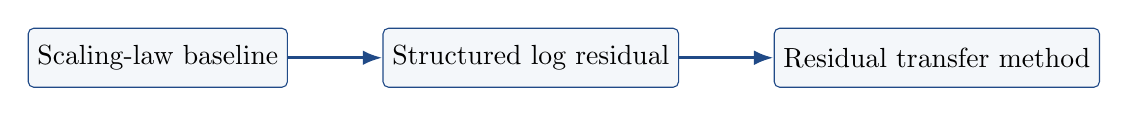
\begin{tikzpicture}[
      node distance=1.2cm,
      box/.style={draw=tdltBlue, rounded corners=2pt, fill=tdltLight, align=center, minimum width=3.1cm, minimum height=0.75cm},
      arrow/.style={-{Latex[length=2.5mm]}, very thick, tdltBlue}
    ]
      \node[box] (a) {Scaling-law baseline};
      \node[box, right=of a] (b) {Structured log residual};
      \node[box, right=of b] (c) {Residual transfer method};
      \draw[arrow] (a) -- (b);
      \draw[arrow] (b) -- (c);
    \end{tikzpicture}
  \end{center}
\end{frame}

\begin{frame}[plain]
  \begin{center}
    \vspace{2.2em}
    {\Large\color{tdltBlue}\textbf{Chapter III}}\\[0.5em]
    {\huge\textbf{Residual Method Development}}\\[0.8em]
    \small Which residual coordinate transfers across schedules, and how should tail geometry enter?
  \end{center}
\end{frame}

\begin{frame}{Residual Target}
  Define the post-momentum residual:
  \[
    r_s(t)=\log L_s(t)-\log \widehat L_{\mathrm{mom},s}(t).
  \]
  Our residual model predicts
  \[
    \log \widehat L_s(t)=
    \log \widehat L_{\mathrm{mom},s}(t)+\widehat r_s(t),
    \qquad
    \widehat L_s(t)=\widehat L_{\mathrm{mom},s}(t)\exp\{\widehat r_s(t)\}.
  \]
  \begin{block}{Why model log residuals?}
    The correction is multiplicative on the original loss scale, which keeps the
    prediction positive and lets the baseline carry the global magnitude of the curve.
  \end{block}
\end{frame}

\begin{frame}{Model Selection Lessons}
  \begin{table}
    \centering
    \scriptsize
    \begin{tabularx}{0.98\textwidth}{lXl}
      \toprule
      candidate residual model & what it tested & outcome\\
      \midrule
      constant shift & scalar bias after momentum & barely improves WSD\\
      feature ridge & hand-crafted LR summaries & weak transfer\\
      high-dimensional local features & more LR history & overfits / worse transfer\\
      raw or normalized \(S_1\) & intrinsic-time residual coordinate & phase-warped\\
      MPL-style hybrid decay & low-rank saturated decay features & small gain only\\
      \bottomrule
    \end{tabularx}
  \end{table}
  \smallnote{These ablations motivate a low-dimensional residual model instead of direct high-dimensional schedule-feature regression.}
\end{frame}

\begin{frame}{Method Pipeline}
  \begin{center}
  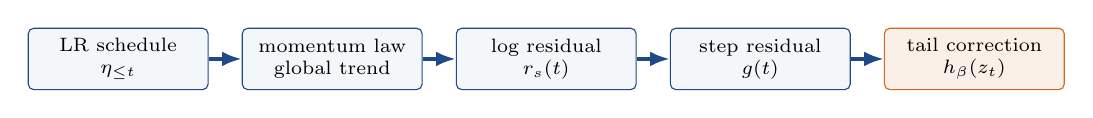
\begin{tikzpicture}[
    node distance=0.42cm,
    box/.style={draw=tdltBlue, rounded corners=2pt, fill=tdltLight, align=center, font=\scriptsize, text width=2.05cm, minimum width=2.15cm, minimum height=0.78cm},
    accent/.style={draw=tdltOrange, rounded corners=2pt, fill=tdltOrange!10, align=center, font=\scriptsize, text width=2.05cm, minimum width=2.15cm, minimum height=0.78cm},
    arrow/.style={-{Latex[length=2.5mm]}, very thick, tdltBlue}
  ]
    \node[box] (x) {LR schedule\\\(\eta_{\le t}\)};
    \node[box, right=of x] (m) {momentum law\\global trend};
    \node[box, right=of m] (r) {log residual\\\(r_s(t)\)};
    \node[box, right=of r] (g) {step residual\\\(g(t)\)};
    \node[accent, right=of g] (h) {tail correction\\\(h_\beta(z_t)\)};
    \draw[arrow] (x) -- (m);
    \draw[arrow] (m) -- (r);
    \draw[arrow] (r) -- (g);
    \draw[arrow] (g) -- (h);
  \end{tikzpicture}
  \end{center}
  \vspace{0.5em}
  \[
    \log \widehat L(t)=
    \log\widehat L_{\mathrm{mom}}(t)+g(t)+h_\beta(z_t).
  \]
  \begin{block}{Modeling principle}
    Keep the scaling-law baseline as the interpretable global component, then add
    only residual terms that are selected on 8-1-1 and evaluated on held-out WSD.
  \end{block}
\end{frame}

\begin{frame}{Method I: Step-Aligned Residual Spline}
  \begin{columns}[T,onlytextwidth]
    \begin{column}{0.52\textwidth}
      Fit a smooth function \(g\) on cosine residuals:
      \[
        g^*=\arg\min_{g\in\mathcal G}
        \sum_{t\in\mathcal T_{\rm cos}}
        (r_{\rm cos}(t)-g(t))^2+\lambda\int |g''(u)|^2du.
      \]
      Transfer:
      \[
      \begin{aligned}
        \log \widehat L_{\rm WSD}(t)
        =&\ \log\widehat L_{\rm mom,WSD}(t)\\
        &+\mathrm{clip}\!\left(\gamma g^*(t),-c,c\right).
      \end{aligned}
      \]
      \small \(g\) is a cubic smoothing spline, \(\lambda\) controls smoothness,
      \(\gamma\) is a shrinkage coefficient, and \(c\) bounds the residual magnitude.
    \end{column}
    \begin{column}{0.44\textwidth}
      
\includegraphics[width=\textwidth]{zijun/method_development/figures/momentum_residual_spline_full.png}
      \smallnote{Visual diagnostic: momentum baseline and smooth residual correction on cosine/WSD sampled trajectories.}
    \end{column}
  \end{columns}
\end{frame}

\begin{frame}{Step Spline Result and Mechanism}
  \begin{columns}[T,onlytextwidth]
    \begin{column}{0.49\textwidth}
      \begin{table}
        \centering
        \scriptsize
        \begin{tabular}{lccc}
          \toprule
          WSD sampled model & MAE & RMSE & \(R^2\)\\
          \midrule
          momentum & 0.037216 & 0.046672 & 0.928180\\
          mean shift & 0.036862 & 0.046243 & 0.929493\\
          spline \(s=0.1\) & \textbf{0.020657} & \textbf{0.024735} & \textbf{0.979827}\\
          \bottomrule
        \end{tabular}
      \end{table}
      \smallnote{Cosine-fitted residual spline transferred to WSD.}
    \end{column}
    \begin{column}{0.49\textwidth}
      \begin{table}
        \centering
        \scriptsize
        \begin{tabular}{lcc}
          \toprule
          coordinate & residual corr. & WSD MAE\\
          \midrule
          absolute step & \textbf{0.936} & \textbf{0.020767}\\
          raw \(S_1\) & -0.123 & 0.045414\\
          \(S_1\) ratio & -0.008 & 0.039812\\
          \bottomrule
        \end{tabular}
      \end{table}
      \smallnote{After momentum correction, residual phase is step-aligned rather than \(S_1\)-aligned.}
    \end{column}
  \end{columns}
\end{frame}

\begin{frame}{Step Spline Robustness}
  \begin{columns}[T,onlytextwidth]
    \begin{column}{0.49\textwidth}
      \begin{block}{Block-resampled improvement}
        \scriptsize
        \begin{tabular}{lccc}
          \toprule
          WSD window & mean \(\Delta\) & q05 & \(P(\Delta>0)\)\\
          \midrule
          full & 0.016843 & 0.010497 & 1.000\\
          tail & 0.016898 & 0.010157 & 1.000\\
          last 2048 & 0.024261 & 0.024261 & 1.000\\
          \bottomrule
        \end{tabular}
      \end{block}
      \smallnote{\(\Delta=|e_{\rm mom}|-|e_{\rm spline}|\); positive values mean the spline reduces absolute error.}
    \end{column}
    \begin{column}{0.49\textwidth}
      \begin{block}{Residual-template controls}
        \scriptsize
        \begin{tabular}{lcc}
          \toprule
          template & full MAE & tail MAE\\
          \midrule
          true step spline & \textbf{0.020878} & \textbf{0.021855}\\
          reversed residual & 0.049905 & 0.047814\\
          circular shift & 0.050053 & 0.051580\\
          block permutation & 0.050067 & 0.049095\\
          sign flip & 0.067432 & 0.067303\\
          \bottomrule
        \end{tabular}
      \end{block}
      \smallnote{Misaligned templates fail, so the gain is tied to residual phase rather than residual magnitude alone.}
    \end{column}
  \end{columns}
\end{frame}

\begin{frame}{Validation Stability of the Step Residual}
  \begin{columns}[T,onlytextwidth]
    \begin{column}{0.52\textwidth}
      \begin{table}
        \centering
        \tiny
        \begin{tabular}{lcccc}
          \toprule
          config & 8-1-1 MAE & WSD MAE & val rank & test rank\\
          \midrule
          \(s=0.01,\lambda=1\) & 0.016447 & 0.020878 & 1 & 1\\
          \(s=0.05,\lambda=1\) & 0.017002 & 0.021281 & 3 & 3\\
          \(s=0.10,\lambda=1\) & 0.017600 & 0.021741 & 5 & 5\\
          \bottomrule
        \end{tabular}
      \end{table}
    \end{column}
    \begin{column}{0.44\textwidth}
      \begin{block}{Selection evidence}
        The 8-1-1 validation ranking closely matches the WSD ranking
        (\(\rho_{\rm Spearman}=0.989\), \(r_{\rm Pearson}=0.997\)).
        The best and conservative spline settings differ by less than
        \(0.001\) WSD MAE.
      \end{block}
    \end{column}
  \end{columns}
  \smallnote{The evidence supports reporting a stable step-residual family, not a fragile single setting.}
\end{frame}

\begin{frame}{Method II: Event/Tail Leftover}
  The step template leaves a small but systematic tail leftover. We fit a
  ridge correction \(h_\beta(z_t)\) on cosine leftover features:
  \[
    \ell_{\rm cos}(t)=r_{\rm cos}(t)-g^*(t),\qquad
    h_\beta(z_t)=\beta_0+\beta^\top\mathrm{standardize}(z_t),
  \]
  \[
    \widehat r_{\rm final}(t)=
    \mathrm{clip}\!\left(g^*(t)+h_\beta(z_t),-c,c\right).
  \]
  \begin{columns}[T,onlytextwidth]
    \begin{column}{0.48\textwidth}
      \begin{block}{Feature vector \(z_t\)}
        \(z_t=(q_t,1-t/T,p_t,p_t^2)\), where \(p_t\) is normalized progress
        through the decay/tail region and \(q_t\) is linear decay progress.
        \(\mathrm{standardize}(\cdot)\) uses cosine statistics.
      \end{block}
    \end{column}
    \begin{column}{0.48\textwidth}
      \begin{alertblock}{Interpretation boundary}
        \(z_t\) is not an optimizer-state measurement. It is a schedule-derived
        proxy for tail geometry; optimizer EMA, weight decay state, weight RMS,
        and update RMS are not observed in the provided data.
      \end{alertblock}
    \end{column}
  \end{columns}
\end{frame}

\begin{frame}{Event/Tail Feature Evidence}
  \begin{columns}[T,onlytextwidth]
    \begin{column}{0.50\textwidth}
      \begin{block}{Incremental information test}
        \scriptsize
        \begin{tabular}{lcc}
          \toprule
          comparison & full MAE & interpretation\\
          \midrule
          step reference & 0.035007 & binned reference\\
          aligned leftover & \textbf{0.029644} & supported\\
          train on 8-1-1 only & 0.030152 & weak transfer\\
          train on cosine+8-1-1 & 0.029322 & supported\\
          \bottomrule
        \end{tabular}
      \end{block}
      \smallnote{The useful correction is schedule-aligned tail geometry on top of the step template.}
    \end{column}
    \begin{column}{0.48\textwidth}
      \begin{block}{Feature-family ablation}
        \scriptsize
        \begin{tabular}{lcc}
          \toprule
          feature family & full MAE & tail MAE\\
          \midrule
          linear endpoint & \textbf{0.029644} & \textbf{0.031012}\\
          drop impulse & 0.033357 & 0.037049\\
          event-tail interactions & 0.034400 & 0.031355\\
          event history & 0.082043 & 0.266411\\
          full event-local & 0.085251 & 0.284405\\
          \bottomrule
        \end{tabular}
      \end{block}
      \smallnote{Low-dimensional endpoint/tail features transfer better than high-dimensional event-history features.}
    \end{column}
  \end{columns}
\end{frame}

\begin{frame}{Methodological Takeaway}
  \begin{block}{What the method development contributes}
    \begin{itemize}
      \item Residual learning is anchored to a reproduced scaling-law baseline.
      \item The first useful residual coordinate is absolute step, not raw or normalized \(S_1\).
      \item The second useful correction is low-rank tail geometry, not arbitrary event-history features.
      \item The method stays testable: cosine fit, 8-1-1 selection, WSD held-out reporting.
    \end{itemize}
  \end{block}
\end{frame}

\begin{frame}[plain]
  \begin{center}
    \vspace{2.2em}
    {\Large\color{tdltBlue}\textbf{Chapter IV}}\\[0.5em]
    {\huge\textbf{Evaluation and Limitations}}\\[0.8em]
    \small How accurate is the final model on held-out WSD, and where are its limits?
  \end{center}
\end{frame}

\begin{frame}{Held-Out WSD Evaluation}
  \begin{table}
    \centering
    \scriptsize
    \begin{tabular}{lccccc}
      \toprule
      WSD test model & full MAE & RMSE & full \(R^2\) & tail MAE & endpoint abs.\\
      \midrule
      momentum baseline & 0.037720 & 0.047275 & 0.926313 & 0.038754 & 0.045668\\
      event decay only & 0.032596 & -- & 0.945083 & 0.032285 & 0.050142\\
      step reference & 0.021281 & 0.025610 & 0.978375 & 0.022268 & \textbf{0.004676}\\
      step + event leftover & \textbf{0.011191} & \textbf{0.014137} & \textbf{0.993410} & \textbf{0.015937} & 0.016615\\
      \bottomrule
    \end{tabular}
  \end{table}
  \begin{block}{Main result}
    The step + event leftover model gives the best full-curve and tail accuracy
    on the held-out WSD schedule, with full-resolution \(R^2=0.993410\).
  \end{block}
\end{frame}

\begin{frame}{Endpoint Behavior Remains a Separate Objective}
  \begin{columns}[T,onlytextwidth]
    \begin{column}{0.48\textwidth}
      \begin{block}{Full/tail gain}
        \[
          \mae_{\rm full}: 0.021281 \to 0.011191
        \]
        \[
          \mae_{\rm tail}: 0.022268 \to 0.015937
        \]
      \end{block}
    \end{column}
    \begin{column}{0.48\textwidth}
      \begin{alertblock}{Endpoint tradeoff}
        \[
          \mathrm{endpoint\ abs.}: 0.004676 \to 0.016615
        \]
        Pure step reference remains better for endpoint behavior.
      \end{alertblock}
    \end{column}
  \end{columns}
  \vspace{0.3em}
  \smallnote{The final claim is therefore about full-curve accuracy, not endpoint optimality.}
\end{frame}

\begin{frame}{Binned Robustness and Ablation}
  \begin{columns}[T,onlytextwidth]
    \begin{column}{0.52\textwidth}
      \begin{table}
        \centering
        \scriptsize
        \begin{tabular}{lcc}
          \toprule
          binned WSD variant & full MAE & tail MAE\\
          \midrule
          step reference & 0.035007 & 0.035694\\
          aligned leftover & \textbf{0.029644} & \textbf{0.031012}\\
          zero event control & 0.035032 & 0.035836\\
          shifted event control & 0.035132 & 0.036998\\
          reverse-time control & 0.038455 & 0.036350\\
          \bottomrule
        \end{tabular}
      \end{table}
    \end{column}
    \begin{column}{0.44\textwidth}
      \begin{block}{Interpretation}
        \begin{itemize}
          \item Aligned event/tail features improve over the step reference.
          \item Zero, shifted, and reversed controls lose the improvement.
          \item The binned experiment is a robustness check; the main metric is the full-resolution WSD result.
        \end{itemize}
      \end{block}
    \end{column}
  \end{columns}
\end{frame}

\begin{frame}{Within-WSD Bootstrap Evidence}
  \begin{table}
    \centering
    \scriptsize
    \begin{tabular}{lcccc}
      \toprule
      window & mean MAE improvement & q05 & q95 & prob. positive\\
      \midrule
      full & 0.005363 & 0.003307 & 0.009138 & 1.000\\
      tail \(27126\)-\(33906\) & 0.004682 & 0.001656 & 0.006967 & 1.000\\
      last 512 & \(-0.000188\) & \(-0.000487\) & \(-0.000090\) & 0.000\\
      \bottomrule
    \end{tabular}
  \end{table}
  \begin{block}{Interpretation}
    Bootstrap supports the full/tail gain within the WSD curve. It does not
    prove schedule-level significance because the independent schedule count is three.
  \end{block}
\end{frame}

\begin{frame}{Overall Method Comparison}
  \begin{columns}[T,onlytextwidth]
    \begin{column}{0.52\textwidth}
      \begin{table}
        \centering
        \scriptsize
        \begin{tabular}{lcc}
          \toprule
          model family & WSD MAE & WSD \(R^2\)\\
          \midrule
          Momentum law & 0.037844 & 0.925669\\
          Multi-Power Law & 0.036027 & 0.935676\\
          residual spline & 0.020657 & 0.979827\\
          step reference & 0.021281 & 0.978375\\
          step + event leftover & \textbf{0.011191} & \textbf{0.993410}\\
          \bottomrule
        \end{tabular}
      \end{table}
    \end{column}
    \begin{column}{0.44\textwidth}
      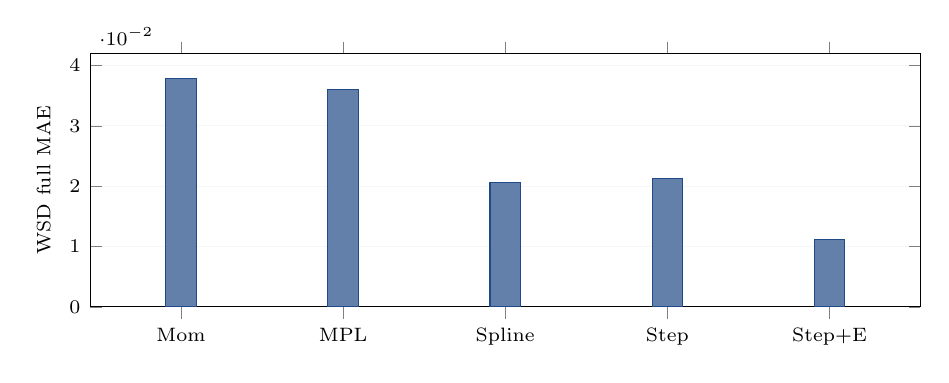
\begin{tikzpicture}
        \begin{axis}[
          ybar,
          width=\textwidth,
          height=4.8cm,
          ymin=0,
          ymax=0.042,
          ylabel={WSD full MAE},
          symbolic x coords={Mom,MPL,Spline,Step,Step+E},
          xtick=data,
          bar width=11pt,
          enlarge x limits=0.14,
          ymajorgrids=true,
          grid style={draw=tdltLight},
          tick label style={font=\scriptsize},
          label style={font=\scriptsize},
        ]
          \addplot[fill=tdltBlue!70,draw=tdltBlue] coordinates {
            (Mom,0.037844)
            (MPL,0.036027)
            (Spline,0.020657)
            (Step,0.021281)
            (Step+E,0.011191)
          };
        \end{axis}
      \end{tikzpicture}
    \end{column}
  \end{columns}
  \smallnote{Some rows use slightly different sampling/reporting contexts; the main comparison follows the cosine-fit, 8-1-1-validation, WSD-test protocol.}
\end{frame}

\begin{frame}{Empirical Findings}
  \begin{columns}[T,onlytextwidth]
    \begin{column}{0.49\textwidth}
      \begin{block}{Supported by experiments}
        \begin{itemize}
          \item Baseline-informed residual correction.
          \item Absolute-step residual phase.
          \item Low-rank linear-tail/event leftover.
          \item Validation-only selection with WSD held out.
        \end{itemize}
      \end{block}
    \end{column}
    \begin{column}{0.49\textwidth}
      \begin{block}{Not supported as main mechanisms}
        \begin{itemize}
          \item Constant residual shift.
          \item Direct high-dimensional schedule features.
          \item Replacing step residual by \(S_1\)-intrinsic time alone.
          \item Event-history features without step alignment.
        \end{itemize}
      \end{block}
    \end{column}
  \end{columns}
\end{frame}

\begin{frame}{Limitations and Future Work}
  \begin{columns}[T,onlytextwidth]
    \begin{column}{0.49\textwidth}
      \begin{block}{Limitations}
        \begin{itemize}
          \item Only three schedules and one model/data scale.
          \item Endpoint remains a separate failure mode.
          \item LR schedule is only a proxy for unobserved optimizer state.
          \item Some reproduction settings are simplified under the available compute budget.
        \end{itemize}
      \end{block}
    \end{column}
    \begin{column}{0.49\textwidth}
      \begin{block}{Next experiments}
        \begin{itemize}
          \item Add explicit endpoint constraints.
          \item Test more model sizes, horizons, and schedules.
          \item Use optimizer-state traces if available.
          \item Replace spline with a constrained dynamics-derived basis.
        \end{itemize}
      \end{block}
    \end{column}
  \end{columns}
\end{frame}

\begin{frame}{Conclusion}
  \begin{center}
    \Large
    A strong loss-curve predictor should use scaling laws as a base layer,\\
    then model only the residual structure that transfers.
  \end{center}
  \vspace{0.9em}
  \begin{columns}[T,onlytextwidth]
    \begin{column}{0.32\textwidth}
      \begin{block}{1. Reproduce}
        Momentum law and Multi-Power Law provide LRS-aware baselines.
      \end{block}
    \end{column}
    \begin{column}{0.32\textwidth}
      \begin{block}{2. Improve}
        Step-aligned residual spline substantially reduces WSD transfer error.
      \end{block}
    \end{column}
    \begin{column}{0.32\textwidth}
      \begin{block}{3. Refine}
        Event leftover reaches WSD full \(R^2=0.993410\), with endpoint caveat.
      \end{block}
    \end{column}
  \end{columns}
\end{frame}

\begin{frame}{Reproducibility}
  \begin{block}{Repository}
    \RepoURL
  \end{block}
  \begin{table}
    \centering
    \scriptsize
    \begin{tabularx}{0.98\textwidth}{l>{\raggedright\arraybackslash}X}
      \toprule
      purpose & implementation location\\
      \midrule
      momentum reproduction & \texttt{code/reproduction\_momentum.py}\\
      Multi-Power Law reproduction & \texttt{code/reproduction\_multi-power\_law/}\\
      residual methods and robustness experiments & \texttt{zijun/method\_development/scripts/}\\
      metrics and selected outputs & \texttt{zijun/method\_development/outputs/}\\
      experiment records & \texttt{zijun/method\_development/experiment\_logs/}\\
      \bottomrule
    \end{tabularx}
  \end{table}
  \smallnote{Local environment used during experiments: \texttt{conda activate tdlt}.}
\end{frame}

\begin{frame}{Division of Labor}
  \begin{table}
    \centering
    \scriptsize
    \begin{tabularx}{0.96\textwidth}{lX}
      \toprule
      member & contribution\\
      \midrule
      \MemberA & Problem framing, literature reading, Tissue et al. momentum-law reproduction, presentation background.\\
      \MemberB & Luo et al. Multi-Power Law reproduction, data processing, baseline comparison, metric validation.\\
      \MemberC & Residual spline, event-leftover method development, validation protocol design, slide integration.\\
      \bottomrule
    \end{tabularx}
  \end{table}
\end{frame}

\begin{frame}{References}
  \scriptsize
  \begin{thebibliography}{9}
    \bibitem{tissue2024}
    Tissue et al. (2024).
    \newblock Scaling law with learning rate annealing.
    \newblock arXiv:2408.11029.

    \bibitem{luo2024}
    Luo et al. (2024).
    \newblock A multi-power law for loss curve prediction across learning rate schedules.
    \newblock NeurIPS 2024 Workshop on Mathematics of Modern Machine Learning.

    \bibitem{li2025}
    Li et al. (2025).
    \newblock Functional scaling laws in kernel regression: loss dynamics and learning rate schedules.
    \newblock arXiv preprint.

    \bibitem{hu2024}
    Hu et al. (2024).
    \newblock Warmup-stable-decay learning-rate schedules.

    \bibitem{bi2024}
    Bi et al. (2024).
    \newblock Multi-step learning-rate schedules for LLM pretraining.
  \end{thebibliography}
\end{frame}

\end{document}
